For eccentric orbits, there are two primary additional physical or computational effects to consider. One is the need for eccentric orbit parameters, expressed in terms of an eccentricity and a semilatus rectum, determined by an energy and an angular momentum. The second is the addition of a time dependent coordinate transformation region between tortoise layers in the middle of the computational grid, containing the position of the particle for all times. In this section, I describe Peter Diener's Fortran code, using Niels Warburton's exact initial conditions for l-modes 0 through 5, and Barry Wardell's effective source, which I have run to produce eccentric orbit output. Similar computations have been done before, using the Discontinuous Galerkin method, by Reference~\cite{time_dependent_coordinate_transformation}, for the gravitational tensor field case; however, the scalar Discontinuous Galerkin case is not yet published.

\section{Orbital parameters}

The orbital parameters of an eccentric orbit in a Schwarzschild space-time are defined through the following conditions.
\begin{equation}
  E^2=\frac{(p-2-2e)(p-2+2e)}{p(p-3-e^2)}
\end{equation}
\begin{equation}
  L^2=\frac{p^2M^2}{p-3-e^2}
\end{equation}
Here, $E$ is the energy and $L$ is the angular momentum. $e$ is the eccentricity and $p$ is the semilatus rectum, which is a dimensionless measure of half the ``width'' of the eccentric orbit. More clearly, $r_{periastron}=\frac{pM}{1+e}$ and $r_{apastron}=\frac{pM}{1-e}$. $\chi$ is a parameter that runs from $0$ to $2\pi$ in one radial cycle (as opposed to $\phi$, which runs from $0$ to $2\pi$ in one angular cycle). In terms of these parameters~\cite{pound_poisson},
\begin{eqnarray}
  r^\prime(\chi)=\frac{pMe\sin(\chi-w)}{[1-e\cos(\chi-w)]^2}\\
  \phi^\prime(\chi)=\sqrt{\frac{p}{p-6-2e\cos\nu}}\\
  t^\prime(\chi)=&\frac{p^2M}{(p-2-2e\cos\nu)(1+e\cos\nu)^2}\nonumber\\
  \frac{d\chi}{dt}=&(\frac{dt}{d\chi})^{-1}
\end{eqnarray}
where $\nu=\chi-w$. For an eccentric orbit, $\chi$ and $\phi$ are evolved using a fourth order Runga Kutta integration using the oscillating orbits framework described in Reference~\ref{pound_poisson}. For a self consistent evolving orbit with the back-reaction effect of the self-force, see future work in Chapter~\ref{futurework}. 


\section{Time dependent coordinate transformation}

In the case of an eccentric orbit, it is necessary to ensure that the particle always remains within the tortoise region, so that the effective source remains valid. We use a time dependent coordinate transformation to keep the particle fixed at a specific coordinate location while the space in its immediate neighborhood evolves. With the proper boundary conditions, enforced by the numeric flux, this simulates a particle on an eccentric orbit and produces the same self-force and the same scalar waves at scri plus. The necessary time dependent coordinate transformation can be found in Reference~\cite{time_dependent_coordinate_transformation}. It transforms from tortoise coordinates, $\xi$, to time dependent coordinates, $x$. The location of the particle $\xi_p(t)$, varies in tortoise coordinates but is fixed in time dependent coordinates ($x_p$). $a$ and $b$ are the boundaries of the time dependent region, in computational coordinates. 
\begin{equation}
  x=a+\frac{x_p-a}{\xi_p-a}(\xi-a)+\frac{(b-\xi_p)(\xi_p-a)-(x_p-a)(b-\xi_p)}{(\xi_p-a)(b-\xi_p)(b-a)}(\xi-a)(\xi-\xi_p)
\end{equation}
I have used Mathematica to confirm the time dependent coordinate wave equation used in Peter Diener's Fortran scalar self-force code. Its time and radial components are
\begin{eqnarray}
\frac{d^2\psi}{dt^2}=&(\frac{dx}{d\xi})^-3[\frac{d^2x}{d\xi^2}-\frac{d^2x}{d\xi^2}(\frac{dx}{dt})^2-2\frac{d^2x}{d\xi dt}\frac{dx}{d\xi}-(\frac{d^2x}{dt^2})^2]\frac{d\psi}{d\xi}\nonumber\\
&+[-1+(\frac{dx}{dt})^2](\frac{dx}{d\xi})^{-2}\frac{d^2\psi}{d\xi^2}\nonumber\\
&-2\frac{dx}{dt}(\frac{dx}{d\xi})^{-1}\frac{d^2\psi}{d\xi dt}
\end{eqnarray}

It is necessary to invert the time dependent transformation and subtract the singular field from the scalar field (and its derivatives) to obtain in-going fluxes at elements just outside the world tube. Similarly, to obtain in-going fluxes inside the world tube, we must transform to time dependent coordinates and subtract the singular field from the scalar field. For outgoing fluxes, addition and subtraction are reversed. 


\section{Orbits}

I have computed four orbits of the system, at DG order 44. Figure~\ref{rorb} shows the radius in Schwarzschild coordinates as a function of time. Figure~\ref{chiorb} shows the sense in which this orbit is eccentric-- if it did not precess, it would form an ellipse. Figure~\ref{phiorb} depicts the physical path of the orbit, including precession. Figure~\ref{precession} demonstrates why precession must exist. The periods of the angular variable $\phi$ and the parameter that governs the rate of radial evolution, $\chi$, are not synchronized.

\begin{figure}
  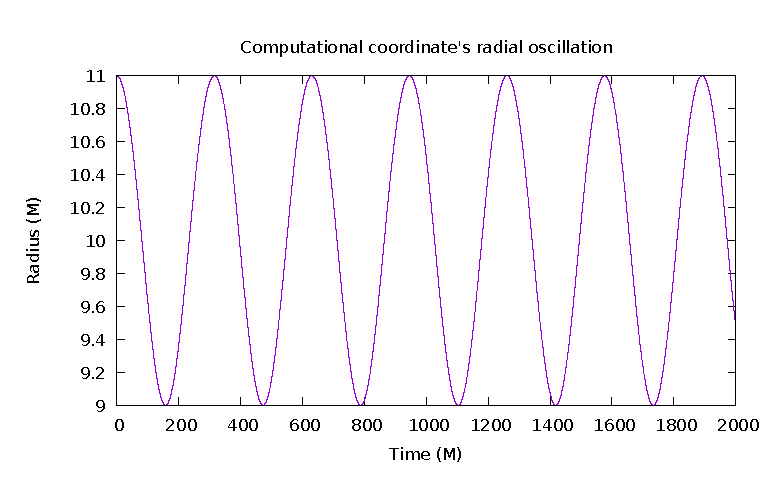
\includegraphics{orbit}
  \caption{Schwarzschild r as a function of time over several orbits.}
  \label{rorb}
\end{figure}


\begin{figure}
  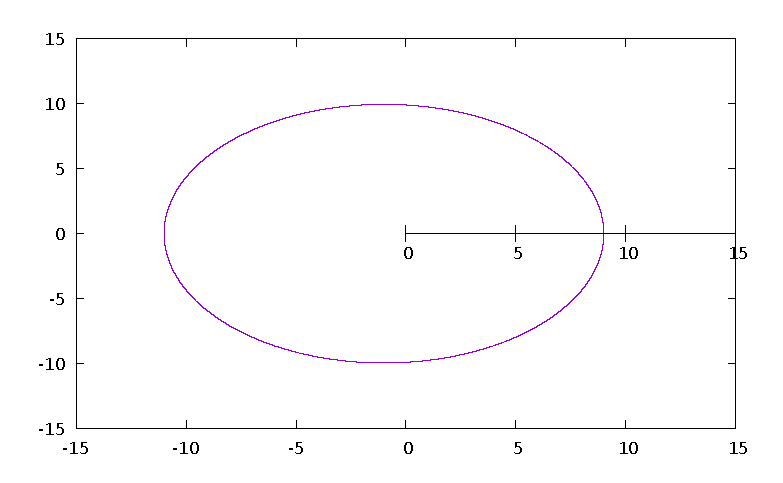
\includegraphics{orbitdg44p99e01}
  \caption{With $\chi$ as the angle in polar coordinates, the orbit forms an exact ellipse. This is the definition of $\chi$, provided r is in Schwarzschild coordinates. Shown for $p=9.9$ and $e=0.1$, DG order 44}
  \label{chiorb}
\end{figure}

\begin{figure}
  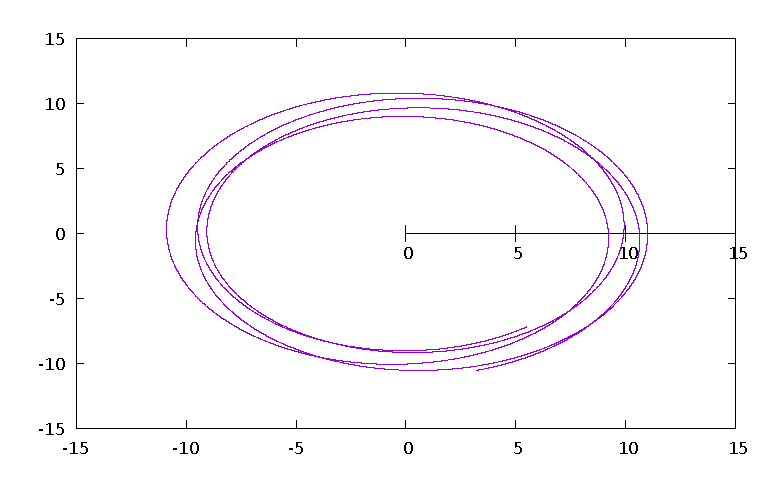
\includegraphics{orbitevolvedg44p99e01}
  \caption{The orbit as it physically would exist, using Schwarzschild $\phi$ as the polar coordinate angle. The orbit precesses but does not inspiral since there is no generic evolution. Shown for $p=9.9$ and $e=0.1$, DG order 44}
  \label{phiorb}
\end{figure}


\begin{figure}
  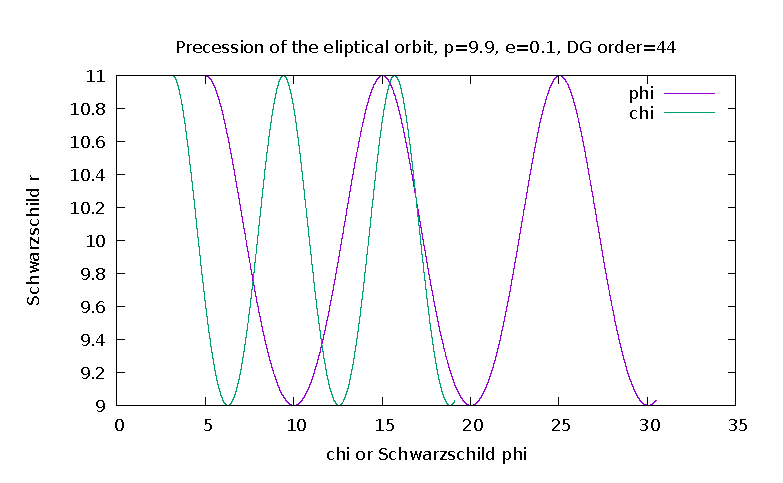
\includegraphics{precessiondg44p99e01}
  \caption{Precession of the eccentric orbit is demonstrated due to the inequality in the period of the angular variables $\chi$, which represents the period of the radial oscillations, and $\phi$, which represents the period of the angular oscillations. $p=9.9$, $e=0.1$, DG order 44.}
  \label{precession}
\end{figure}

\section{Self force output}

The radial self-force is defined as $q\nabla^\alpha\Psi^{R}$~\cite{wardell_vega_thornburg_diener}. To compute this self force, it is necessary to sum over all l and m modes. In principle it is necessary to sum to $l=\infty$. Figures~\ref{rsf},~\ref{tsf}, and~\ref{phisf} are computed using a fit to extrapolate to infinite $l$, based on an analytic sum of the remaining terms after the highest l-mode computed. See Chapter~\ref{sigmachap} for details of the mode sum. Two terms of the sum described in that chapter were used in the fit.


\begin{figure}
  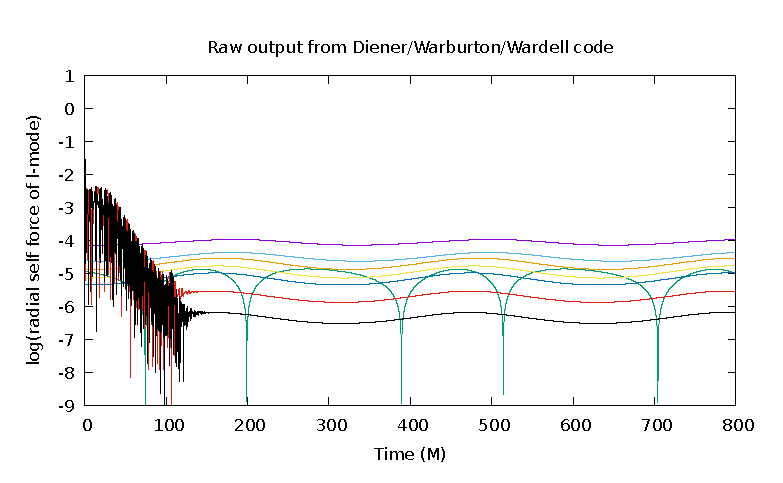
\includegraphics{rawRadialSelForceModes}
  \caption{Raw output of Diener, Warburton, and Wardell code for DG order 44. Radial self force.}
  \label{rsf}
\end{figure}

\begin{figure}
  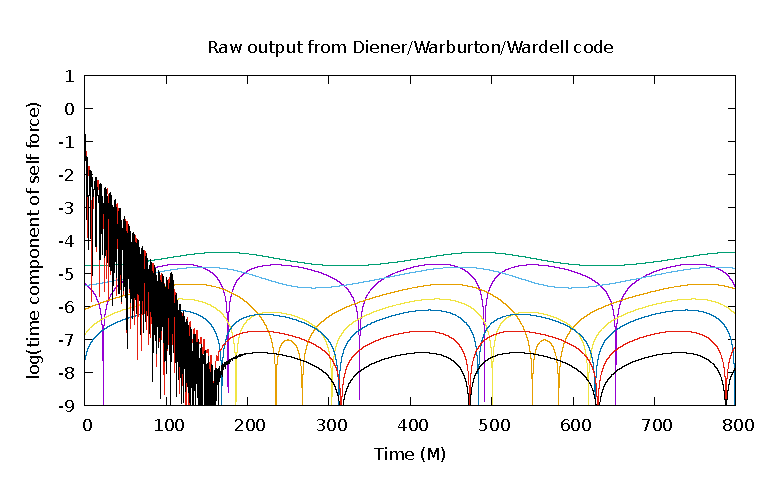
\includegraphics{rawTimeSelfForceModes}
  \caption{Raw output of Diener, Warburton, and Wardell code for DG order 44. Time component of the self force.}
  \label{tsf}
\end{figure}

\begin{figure}
  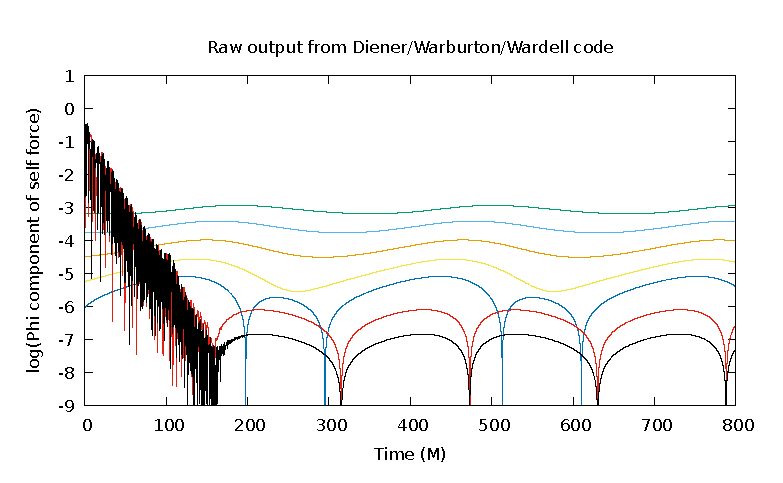
\includegraphics{rawPhiSelfForceModes}
  \caption{Raw output of Diener, Warburton, and Wardell code for DG order 44. Phi component of the self force.}
  \label{phisf}
\end{figure}

